\chapter{Modelo-Vista-Controlador}

La arquitectura \textbf{Modelo-Vista-Controlador} es un patrón de diseño de software que separa las funciones que el software realiza en tres capas principales:

\begin{itemize}
    \item \textbf{Modelo de datos}: Es la representación de la información que la que la aplicación interactúa, tanto para obtener la información como para ser actualizada.

    El modelo de datos normalmente equivale al diseño de base de datos, donde cada modelo representa a una entidad en un diseño de base de datos relacional.

    El controlador es el encargado de realizar las peticiones al modelo, ya se actualizaciones o la obtención de información.

    \item \textbf{Controlador}: Responde a acciones del usuario (o eventos), que normalmente desencadenan en una acción al modelo de datos (ya sea obtención de datos, actualización, borrado...).

    El controlador hace de intermediario entre la vista y el modelo.

    \item \textbf{Vista}: Es la parte que muestra al usuario los datos obtenidos y con la que este interactúa. Esta interacción generará posibles acciones que irán al controlador para volver a empezar el ciclo.
\end{itemize}

\section{Interacción de los componentes}

Aunque existen distintas implementaciones de la arquitectura Modelo-Vista-Controlador, el flujo de acciones suele ser similar al siguiente:

{
\begin{minipage}{0.56\linewidth}
\begin{enumerate}
    \item El usuario interactúa con la interfaz de usuario de alguna forma (por ejemplo, el usuario pulsa un botón, enlace, etc.).

    \item El controlador recibe (por parte de los objetos de la interfaz-vista) la notificación de la acción solicitada por el usuario. El controlador gestiona el evento que llega, frecuentemente a través de un gestor de eventos (handler) o callback.

    \item El controlador realiza una petición al modelo, ya sea para solicitar información o para actualizarla. El modelo debe confirmar si la acción se ha realizado de manera correcta o no.

    \item El controlador delega en la vista la información obtenida para que sea visualizada.

    \item La interfaz se mantiene a la espera de una nueva interacción para comenzar de nuevo el ciclo.
\end{enumerate}
\end{minipage}
\hfill
\begin{minipage}{0.4\linewidth}
    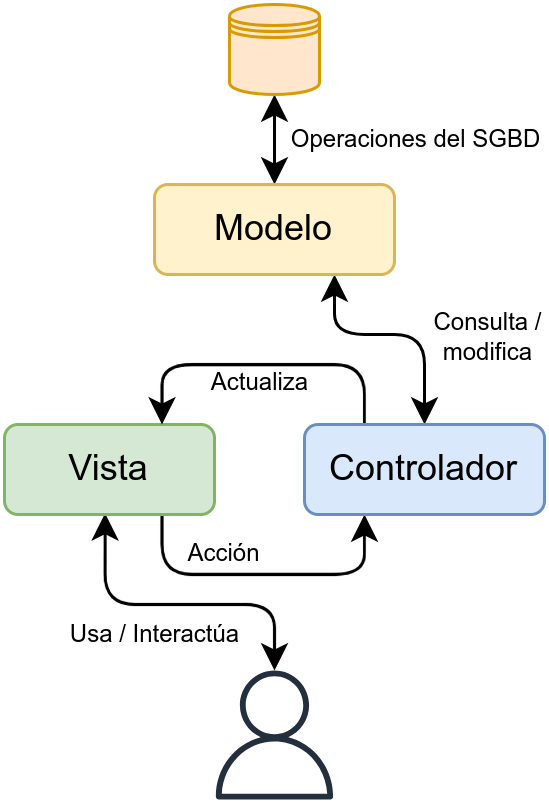
\includegraphics[width=\linewidth]{mvc.png}
\end{minipage}
}

\vspace{10pt}
Tal como se ha dicho, pueden existir distintas implementaciones, pero de manera generalizada y simplificada este sería el esquema básico de interacción.


\chapter{ORM}
Los sistemas ORM (del inglés \textit{Object-Relational mapping}, o “mapeo objeto-relacional”) es una técnica de programación para convertir los datos de una base de datos relacional en objetos cuando son utilizados en un lenguaje de programación orientado a objetos.

Este sistema “simula” una base de datos orientada a objetos (que no están muy extendidas) haciendo uso de las bases de datos relacionales que son ampliamente utilizadas y son más conocidas. De esta manera, también es un sistema menos a mantener.

Estos sistemas ORM suelen ocultar cómo se generan las peticiones a la base de datos, ya que para el programador lo único que hace es interactuar con objetos. El motor que usa Laravel se llama \href{https://laravel.com/docs/10.x/eloquent#retrieving-models}{Eloquent}.

Muchos \textit{framewors} de programación hacen uso de sistemas ORM, por lo que dependerá de cuál usemos podremos hacer uso de uno o podremos elegir entre varios. La wikipedia tiene una página donde se \href{https://en.wikipedia.org/wiki/List_of_object%E2%80%93relational_mapping_software}{listan distintos ORMs} separados por lenguajes de programación.